% Options for packages loaded elsewhere
\PassOptionsToPackage{unicode}{hyperref}
\PassOptionsToPackage{hyphens}{url}
%
\documentclass[
  12pt,
  oneside]{book}
\usepackage{amsmath,amssymb}
\usepackage{lmodern}
\usepackage{setspace}
\usepackage{iftex}
\ifPDFTeX
  \usepackage[T1]{fontenc}
  \usepackage[utf8]{inputenc}
  \usepackage{textcomp} % provide euro and other symbols
\else % if luatex or xetex
  \usepackage{unicode-math}
  \defaultfontfeatures{Scale=MatchLowercase}
  \defaultfontfeatures[\rmfamily]{Ligatures=TeX,Scale=1}
\fi
% Use upquote if available, for straight quotes in verbatim environments
\IfFileExists{upquote.sty}{\usepackage{upquote}}{}
\IfFileExists{microtype.sty}{% use microtype if available
  \usepackage[]{microtype}
  \UseMicrotypeSet[protrusion]{basicmath} % disable protrusion for tt fonts
}{}
\usepackage{xcolor}
\IfFileExists{xurl.sty}{\usepackage{xurl}}{} % add URL line breaks if available
\IfFileExists{bookmark.sty}{\usepackage{bookmark}}{\usepackage{hyperref}}
\hypersetup{
  hidelinks,
  pdfcreator={LaTeX via pandoc}}
\urlstyle{same} % disable monospaced font for URLs
\usepackage[left=1in, right=1in, top=1in, bottom=1in]{geometry}
\usepackage{color}
\usepackage{fancyvrb}
\newcommand{\VerbBar}{|}
\newcommand{\VERB}{\Verb[commandchars=\\\{\}]}
\DefineVerbatimEnvironment{Highlighting}{Verbatim}{commandchars=\\\{\}}
% Add ',fontsize=\small' for more characters per line
\usepackage{framed}
\definecolor{shadecolor}{RGB}{248,248,248}
\newenvironment{Shaded}{\begin{snugshade}}{\end{snugshade}}
\newcommand{\AlertTok}[1]{\textcolor[rgb]{0.94,0.16,0.16}{#1}}
\newcommand{\AnnotationTok}[1]{\textcolor[rgb]{0.56,0.35,0.01}{\textbf{\textit{#1}}}}
\newcommand{\AttributeTok}[1]{\textcolor[rgb]{0.77,0.63,0.00}{#1}}
\newcommand{\BaseNTok}[1]{\textcolor[rgb]{0.00,0.00,0.81}{#1}}
\newcommand{\BuiltInTok}[1]{#1}
\newcommand{\CharTok}[1]{\textcolor[rgb]{0.31,0.60,0.02}{#1}}
\newcommand{\CommentTok}[1]{\textcolor[rgb]{0.56,0.35,0.01}{\textit{#1}}}
\newcommand{\CommentVarTok}[1]{\textcolor[rgb]{0.56,0.35,0.01}{\textbf{\textit{#1}}}}
\newcommand{\ConstantTok}[1]{\textcolor[rgb]{0.00,0.00,0.00}{#1}}
\newcommand{\ControlFlowTok}[1]{\textcolor[rgb]{0.13,0.29,0.53}{\textbf{#1}}}
\newcommand{\DataTypeTok}[1]{\textcolor[rgb]{0.13,0.29,0.53}{#1}}
\newcommand{\DecValTok}[1]{\textcolor[rgb]{0.00,0.00,0.81}{#1}}
\newcommand{\DocumentationTok}[1]{\textcolor[rgb]{0.56,0.35,0.01}{\textbf{\textit{#1}}}}
\newcommand{\ErrorTok}[1]{\textcolor[rgb]{0.64,0.00,0.00}{\textbf{#1}}}
\newcommand{\ExtensionTok}[1]{#1}
\newcommand{\FloatTok}[1]{\textcolor[rgb]{0.00,0.00,0.81}{#1}}
\newcommand{\FunctionTok}[1]{\textcolor[rgb]{0.00,0.00,0.00}{#1}}
\newcommand{\ImportTok}[1]{#1}
\newcommand{\InformationTok}[1]{\textcolor[rgb]{0.56,0.35,0.01}{\textbf{\textit{#1}}}}
\newcommand{\KeywordTok}[1]{\textcolor[rgb]{0.13,0.29,0.53}{\textbf{#1}}}
\newcommand{\NormalTok}[1]{#1}
\newcommand{\OperatorTok}[1]{\textcolor[rgb]{0.81,0.36,0.00}{\textbf{#1}}}
\newcommand{\OtherTok}[1]{\textcolor[rgb]{0.56,0.35,0.01}{#1}}
\newcommand{\PreprocessorTok}[1]{\textcolor[rgb]{0.56,0.35,0.01}{\textit{#1}}}
\newcommand{\RegionMarkerTok}[1]{#1}
\newcommand{\SpecialCharTok}[1]{\textcolor[rgb]{0.00,0.00,0.00}{#1}}
\newcommand{\SpecialStringTok}[1]{\textcolor[rgb]{0.31,0.60,0.02}{#1}}
\newcommand{\StringTok}[1]{\textcolor[rgb]{0.31,0.60,0.02}{#1}}
\newcommand{\VariableTok}[1]{\textcolor[rgb]{0.00,0.00,0.00}{#1}}
\newcommand{\VerbatimStringTok}[1]{\textcolor[rgb]{0.31,0.60,0.02}{#1}}
\newcommand{\WarningTok}[1]{\textcolor[rgb]{0.56,0.35,0.01}{\textbf{\textit{#1}}}}
\usepackage{longtable,booktabs,array}
\usepackage{calc} % for calculating minipage widths
% Correct order of tables after \paragraph or \subparagraph
\usepackage{etoolbox}
\makeatletter
\patchcmd\longtable{\par}{\if@noskipsec\mbox{}\fi\par}{}{}
\makeatother
% Allow footnotes in longtable head/foot
\IfFileExists{footnotehyper.sty}{\usepackage{footnotehyper}}{\usepackage{footnote}}
\makesavenoteenv{longtable}
\usepackage{graphicx}
\makeatletter
\def\maxwidth{\ifdim\Gin@nat@width>\linewidth\linewidth\else\Gin@nat@width\fi}
\def\maxheight{\ifdim\Gin@nat@height>\textheight\textheight\else\Gin@nat@height\fi}
\makeatother
% Scale images if necessary, so that they will not overflow the page
% margins by default, and it is still possible to overwrite the defaults
% using explicit options in \includegraphics[width, height, ...]{}
\setkeys{Gin}{width=\maxwidth,height=\maxheight,keepaspectratio}
% Set default figure placement to htbp
\makeatletter
\def\fps@figure{htbp}
\makeatother
\setlength{\emergencystretch}{3em} % prevent overfull lines
\providecommand{\tightlist}{%
  \setlength{\itemsep}{0pt}\setlength{\parskip}{0pt}}
\setcounter{secnumdepth}{5}
\usepackage{booktabs}
\pagestyle{plain}
\ifLuaTeX
  \usepackage{selnolig}  % disable illegal ligatures
\fi
\usepackage[]{natbib}
\bibliographystyle{apalike}

\title{Bayesian Inference with Stan\\
for Hybrid Species Distribution Modeling}
\usepackage{etoolbox}
\makeatletter
\providecommand{\subtitle}[1]{% add subtitle to \maketitle
  \apptocmd{\@title}{\par {\large #1 \par}}{}{}
}
\makeatother
\subtitle{\hfill\break
\vspace{+20truemm}\\
Isaac William Caruso\\
Advisor: Prof.~Matteo Riondato\\
April 26, 2021}
\author{\vspace{+45truemm}\\
Submitted to the Department of Computer Science of Amherst College\\
in partial fulfillment of the requirements for the degree of\\
Bachelor of Arts with Distinction}
\date{}

\usepackage{amsthm}
\newtheorem{theorem}{Theorem}[chapter]
\newtheorem{lemma}{Lemma}[chapter]
\newtheorem{corollary}{Corollary}[chapter]
\newtheorem{proposition}{Proposition}[chapter]
\newtheorem{conjecture}{Conjecture}[chapter]
\theoremstyle{definition}
\newtheorem{definition}{Definition}[chapter]
\theoremstyle{definition}
\newtheorem{example}{Example}[chapter]
\theoremstyle{definition}
\newtheorem{exercise}{Exercise}[chapter]
\theoremstyle{remark}
\newtheorem*{remark}{Remark}
\newtheorem*{solution}{Solution}
\begin{document}
\maketitle

{
\setcounter{tocdepth}{1}
\tableofcontents
}
\setstretch{1.7}
\hypertarget{abstract}{%
\chapter*{Abstract}\label{abstract}}
\addcontentsline{toc}{chapter}{Abstract}

Bayesian inference is a statistical technique for estimating a quantity of interest from data.
Increasingly, Bayesian inference is being applied to problems in a variety of fields of study as it allows for the explicit incorporation of \emph{a priori}, \emph{domain-specific} knowledge into the learning process.
While generally appealing for numerous reasons, it has until recently been an impractical tool for learning the parameters of complex, real-world systems.
In this work, we first provide the theoretical concepts necessary for appreciating Bayesian inference.
We then describe algorithms for performing Bayesian inference with computing machines in a computationally feasible manner, namely Metropolis-Hastings Markov Chain Monte Carlo (MCMC).
This is then followed by a discussion of Stan, a domain-specific programming language often used for MCMC and Bayesian inference.
Finally, we conclude this work with a case study from a recent publication in the field of biology, which applies Bayesian inference to the task of species distribution modeling.
Not only is this task extremely pertinent as it relates directly to climate change, but also the resulting model was sufficiently complex to test the full capabilities of the Stan language.

\hypertarget{acknowledgments}{%
\chapter*{Acknowledgments}\label{acknowledgments}}
\addcontentsline{toc}{chapter}{Acknowledgments}

I would like to thank all of the Amherst College Computer Science Department---especially my thesis advisor Professor Matteo Riondato---for facilitating my academic growth over the past four years and in the endeavor of completing this thesis.
Moreover, I thank Professor Lauren Buckley from the University of Washington Department of Biology for graciously providing her expertise and guidance in Biology and Functional Ecology.
I also am excited to acknowledge my parents for their continued support over the entirety of my educational career and my friends, who provided an extensive network of support during my time at Amherst.

\hypertarget{introduction}{%
\chapter*{Introduction}\label{introduction}}
\addcontentsline{toc}{chapter}{Introduction}

As data collection becomes increasingly commonplace, extracting meaning from large datasets is essential for drawing insights and predictions.
Understanding how a large number of factors influence a dataset is a topic of certain relevance for almost every scientific domain.
In the field of biology, as we expand upon in the fourth chapter, understanding where animal species occur in the wild and how these ranges are shifting over time due to environmental factors is of critical importance for conservation efforts to have the greatest possible effect.
Conservation biologists and ecologists have been studying these species' tolerances to the environment for quite some time, so we understand how different properties of the environment influence the occurrence of species we are interested in.
Additionally, we are not only interested in where these species have been observed, but also where they have \emph{not} been observed.
The fields of statistics and machine learning provides the computational tools necessary for addressing this inquiry and many others.
Given existing data, we learn a \emph{model} which incorporates information we already have and the data we have available to us to predict what a situation for which we do not yet have the data will look like.
As we elaborate upon in the first chapter of this work, Bayesian approaches to learning allow us to incorporate \emph{a priori} domain-specific knowledge in a manner that is both explicit and intuitive.
The second chapter discusses \emph{Markov Chain Monte Carlo} (MCMC) and related algorithmic developments that make Bayesian inference feasible and scalable.
Chapter three presents a discussion of Stan, a software project aimed at making Bayesian inference fast and accessible.
Since at the outset Bayesian inference may appear quie complex, we aim to provide a gradual introduction first to probability and the concepts necessary to comprehend Bayesian statistics and secondly to how performing Bayesian inference is possible using modern computational techniques.

\hypertarget{probability-primer}{%
\chapter{Probability primer}\label{probability-primer}}

This chapter provides an introduction to the probability concepts necessary to understand Bayesian inference.
Simply put, Bayesian inference is a statistical technique for estimating a quantity of interest upon the observation of data, while explicitly incorporating \emph{prior knowledge or belief} about that quantity of interest.
Before embarking on an exposition of Bayesian statistics, we must first gain a basic understanding of a few key elements of probability theory---random variables, cumulative distribution functions, probability functions/ distributions, expected value, and conditional probability.
This chapter concludes by introducing Bayes' theorem and Bayesian inference.

\hypertarget{random-variables}{%
\section{Random Variables}\label{random-variables}}

Imagine for a moment you are tossing a fair coin.
There are many experiments you could perform by tossing a coin, but let us consider our quantity of interest to be the fraction of times our coin lands on a tail.
It is clear that the number of tails, the outcome of our experiment, is dependent on the eventual realization of some random process.
A \emph{random variable} \(X\) is a variable whose value is dependent on the outcome(s) of a stochastic phenomenon.
The realized value of \(X\) is denoted as \(x\).

In the example of tossing a coin, where the data is a sequence of coin tosses, e.g., \([H, T, T, …]\), we define the random variable \(X\) to be the number of tails.
If we toss the coin twice, \(X\) has three possible realized states, \(x\), depending on the outcome of this stochastic experiment: \(x = 0\), \(x = 1\), or \(x = 2\).
Table \ref{tab:rv} shows the probability that our random variable \(X\) takes value \(x\), some actual number of tails.

\begin{table}[!h]

\caption{\label{tab:rv}P(X = x) for two tosses}
\centering
\begin{tabular}[t]{rr}
\toprule
x & P(X = x)\\
\midrule
0 & 0.25\\
1 & 0.50\\
2 & 0.25\\
\bottomrule
\end{tabular}
\end{table}

The r.v. \(X\) is is an example of a \emph{discrete random variable}.
Discrete random variables can only assume discrete values.
On the contrary, continuous random variables are useful for describing continuous sample spaces.
For example, a continuous random variable may be used to represent the outcome of an experiment measuring blossoming heights of flowers, where the data is a sequence of observations of heights at which different flowers blossomed.
In this case, the outcome of our blossoming experiment can be any of an infinite number of real values, thus is properly modeled by a continuous random variable.

\hypertarget{cumulative-distribution-functions}{%
\section{Cumulative Distribution Functions}\label{cumulative-distribution-functions}}

In the previous example, we represented the probability of various outcomes of a coin toss experiment in a tabular format.
Another way to represent this set of probabilities is as a \emph{cumulative distribution function} \citep[ \text{Sec} 2.2]{Wasserman2004}.

\begin{definition}[Cumulative distribution function 'CDF']
\protect\hypertarget{def:cdf}{}{\label{def:cdf} \iffalse (Cumulative distribution function `CDF') \fi{} }\emph{The cumulative distribution function is defined as the function}
\[F_{X}(x) \doteq P(X≤x)\]
\end{definition}

The cumulative distribution function \(F_{X}(x)\) simply represents the probability that a random variable \(X\) takes a value less than or equal to \(x\) for each possible input value of \(x\).
Figure \ref{fig:cdfimg} depicts a graphical representation of the CDF for our coin-tossing experiment.



\begin{figure}

{\centering 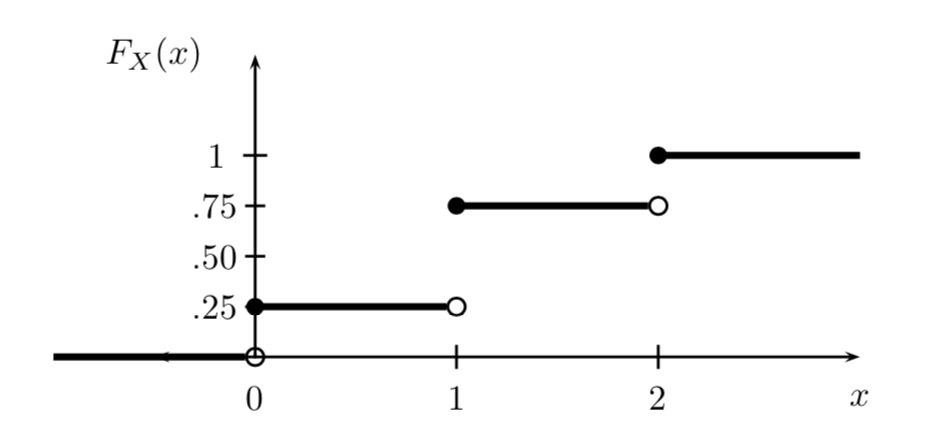
\includegraphics[width=0.7\linewidth]{./images/cdf} 

}

\caption{CDF for tossing a coin twice \citep[ \text{Sec} 2.2]{Wasserman2004}}\label{fig:cdfimg}
\end{figure}

Here, for every value of \(x\)---the number of tails in two coin tosses---the probability that \(X\) is equal to or less than this value is represented.
In this discrete example, we see that our CDF is represented by several non-decreasing discrete lines defined for all \(x\).
In the example of a continuous random variable, this function is a non-decreasing distribution also defined for all \(x\).

\hypertarget{probability-mass-and-density-functions}{%
\section{Probability Mass and Density Functions}\label{probability-mass-and-density-functions}}

The \emph{probability mass function} (PMF) and \emph{probability density function} (PDF) allow us to express probabilities of events over a sample space and find their use with discrete and continuous random variables respectively.

In the discrete setting, the probability mass function for a random variable \(X\) yields the probability that \(X\) takes a value \(x\) for every possible value that \(X\) can take \citep[ \text{Sec} 2.2]{Wasserman2004}.

\begin{definition}[Probability mass function 'PMF']
\protect\hypertarget{def:pmf}{}{\label{def:pmf} \iffalse (Probability mass function `PMF') \fi{} }\emph{The probability function for a discrete random variable \(X\)---known as the }probability mass function* for \(X\)---is defined as the function*
\[f_{X}(x) \doteq P(X=x)\]
\end{definition}

Here, the PMF has a few key attributes.
Namely \(P(X=x)>0\) for every \(x\) in the sample space \(S_{X}\) of \(X\), and \(\sum_{x \in S_{X}}f_{X}(x)=1\).
With these features in mind, the probability mass function of \(X\) follows logically from the cumulative distribution function of \(X\) insofar as the CDF is the sum of the PMF for all \(x_{i}≤x\) \citep[ \text{Sec} 2.2]{Wasserman2004}, i.e., \[F_{X}(x) \doteq P(X≤x)=\sum_{x_i≤x}f_{X}(x_{i}).\]

In the case where the random variable \(X\) is continuous, its probability density function is defined as follows \citep[ \text{Sec} 2.2]{Wasserman2004}.

\begin{definition}[Probability density function 'PDF']
\protect\hypertarget{def:pdf}{}{\label{def:pdf} \iffalse (Probability density function `PDF') \fi{} }\emph{The probability function for a continuous random variable \(X\)---known as the }probability density function* for \(X\)---is defined as a function \(f(x)\) where \(a\) and \(b\) are two real numbers such that \(a ≤ b\), so*
\[P(a<X<b) \doteq \int_{a}^{b}f_X(x)dx.\]
\end{definition}

In other words, the probability that the realized value \(x\) of our continuous random variable \(X\) is between two numbers \(a\) and \(b\) is equal to the integral of the probability density function of \(x\) from \(x = a\) to \(x = b\).
This formalization of the PDF \(f_X(x)\) allows a natural comparison with the CDF \(F_X(x)\) of \(X\),

\[F_X(x) \doteq \int_{-\infty}^{x}f_X(x)dx.\]

Specifically, this implies that \(F'_X(x)=f_X(x)\) for all differentiable points of \(F_X\).
In plain English, this signifies that the derivative of the CDF is the PDF.

\hypertarget{expectation}{%
\section{Expectation}\label{expectation}}

One of the final core probability concepts necessary to approach Bayesian statistics on sure footing is the idea of expectation or expected value \citep[ \text{Sec} 3.1]{Wasserman2004}.

\begin{definition}[Expectation]
\protect\hypertarget{def:e}{}{\label{def:e} \iffalse (Expectation) \fi{} }\emph{The expectation or expected value of a random variable X is}
\[E(X) \doteq \begin{cases}\sum_{x}xf_{X}(x) & \textrm{if }X\textrm{ is discrete}\\\int{xf_{X}(x)dx} & \textrm{if }X\textrm{ is continuous}\end{cases}\]
\end{definition}

To return to a familiar example, consider a random variable \(X\) to represent the number of tails in 6 coin tosses. Figure \ref{fig:binom} depicts the PMF for \(X\) using the \emph{binomial distribution} \(B(6,0.5)\) which represents the probability of observing a specific number of successes in a success-failure experiment, where the probability of success is 0.5.

\begin{figure}

{\centering 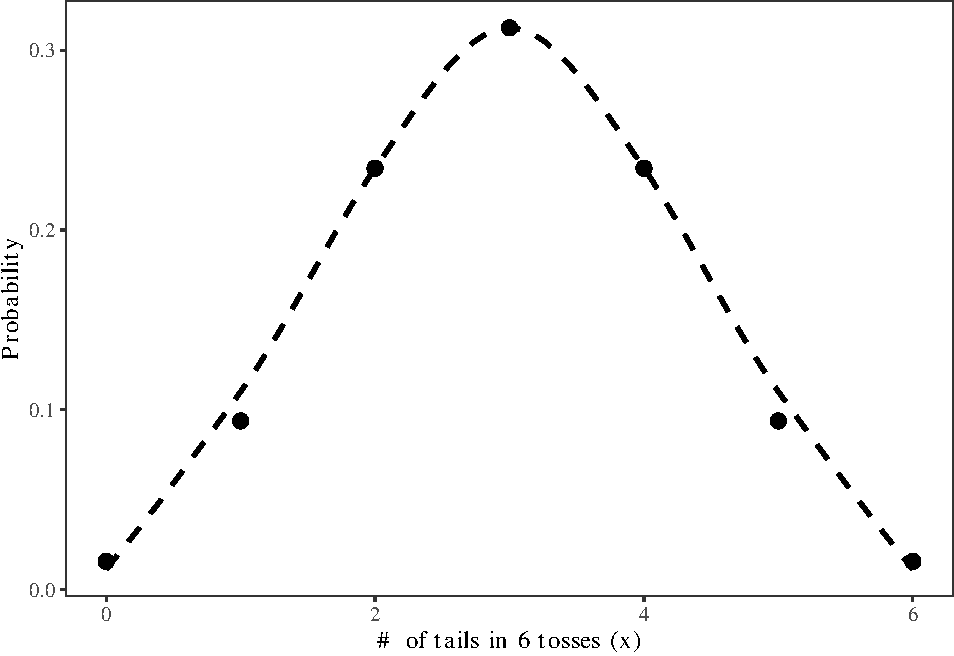
\includegraphics[width=0.5\linewidth]{manuscript_files/figure-latex/binom-1} 

}

\caption{The binomial probability mass function for the 6 trial coin toss experiment}\label{fig:binom}
\end{figure}

In this case, the x-axis represents each possible outcome \(x\) and the y-axis is the probability of that outcome. Table \ref{tab:bino} presents the value of the binomial PMF for every \(x \in X\).

\begin{table}[!h]

\caption{\label{tab:bino}P(X = x) for six tosses}
\centering
\begin{tabular}[t]{rr}
\toprule
x & y\\
\midrule
0 & 0.016\\
1 & 0.094\\
2 & 0.234\\
3 & 0.312\\
4 & 0.234\\
5 & 0.094\\
6 & 0.016\\
\bottomrule
\end{tabular}
\end{table}

Computing \(E(X)\) given the values in this table is demonstrated using the discrete case of Definition \ref{def:e} in Example \ref{exm:coin}.

\begin{example}
\protect\hypertarget{exm:coin}{}{\label{exm:coin} }The expected value of \(X \sim B(6, 0.5)\),
\[\begin{split}
E(X) & = \sum_{x}xf(x) \\
  & =  (0 \times 0.16)+(1 \times 0.094)+(2 \times 0.234)+(3 \times 0.312)\\
  & \;\;\;\; +(4 \times 0.234)+(5 \times 0.094)+(6 \times 0.016)\\
  & = 3
\end{split}\]
\end{example}

Importantly while in this case, \(E(X)\) corresponds well to the ``peak'' in the PMF, this should not be assumed to be the case unilaterally, as the same expectation would result from any distribution symmetrical about \(x=3\).

\hypertarget{conditional-probability}{%
\section{Conditional Probability}\label{conditional-probability}}

\emph{Conditional probability} provides a way to model the probability that an event occurs, given that another event is known to have occurred.
Conditional probability, as presented in Definition \ref{def:condprob}, requires only that the event assumed to have occurred, i.e., the event we are \emph{conditioning on} has a nonzero probability of occurring \citep[ \text{Sec} 3.5]{Wasserman2004}.

\begin{definition}[Conditional Probability]
\protect\hypertarget{def:condprob}{}{\label{def:condprob} \iffalse (Conditional Probability) \fi{} }\emph{Assuming \(P(B)>0\),}
\[P(A|B)=\frac{P(A \cap B)}{P(B)}\]
\end{definition}

Conditional probability asserts that the probability of event A occurring given that event B occurs is equivalent to the probability of both A and B occurring (denoted as \(A \cap B\)) divided by the probability that B occurs. \(P(A|B)\) is not generally equal to \(P(B|A)\).
For example, the probability that I am swimming given that I am in the water is clearly not the same as the probability that I am in the water given that I am swimming.
Example \ref{exm:condprobe} explains how to use conditional probability to calculate the probability of rolling a 2 on a 6-sided dice, given I know the outcome of the roll is less than 4.

\begin{example}
\protect\hypertarget{exm:condprobe}{}{\label{exm:condprobe} }Conditional probability can be used to determine the probability of rolling a 2 on a 6 sided dice, given that I know the outcome will be less than 4. This scenario can be represented as:
\[A = \textrm{rolls 2, } P(A) = 1/6\]
\[B = \textrm{rolls < 4, } P(B) = 3/6\]
\[P(A \cap B) = P(A) = 1/6\]
\[\begin{split}
P(2|<4) = P(A|B) & = \frac{P(A \cap B)}{P(B)} \\
  & = \frac{\frac{1}{6}}{\frac{3}{6}} \\
  & = \frac{1}{3}
\end{split}\]
\end{example}

\hypertarget{bayes-theorem}{%
\section{Bayes' Theorem}\label{bayes-theorem}}

Consider a student, Alice, who was exposed to someone with COVID-19.
Being a responsible citizen, Alice decides she should get tested.
She receives a test and the accompanying information sheet states the test is 85\% accurate, meaning that 85\% of the time it gives positive results to recipients who are actually positive. The sheet also says that the test yields a false positive 30\% of the time, meaning that if Alice is actually negative she will still receive a positive test 30\% of the time.
The following day Alice receives a positive test.
As a student of probability, Alice recognizes that the 85\% accuracy statistic only means the conditional probability that she receives a positive test given she is COVID positive (\(P(+ test|covid+)\)) is 85\%.
However, Alice is really interested in the conditional probability that she is positive given she just tested positive, \(P(covid+|test+)\).
As stated in the previous section's discussion of conditional probability, \(P(A|B) \neq P(B|A)\).
\emph{Bayes' theorem}, which follows intuitively from the theorem of conditional probability, provides this answer for Alice.
We can rewrite Definition \ref{def:condprob} as
\[P(A \cap B)=P(A|B)P(B).\]
Furthermore, it can also be stated that
\[P(B \cap A)=P(B|A)P(A)\]
Clearly, \(P(A \cap B)=P(B \cap A)\) as both notations can be used interchangeably to represent the intersection of two sets A and B.
This identity means that we can rewrite the previous equations as
\[P(B|A)P(A)=P(A|B)P(B)\]
Moreover, dividing both sides of this equivalency by \(P(A)\) yields Bayes' theorem, as formalized in Definition \ref{def:bayestheorem} \citep{Junker2003}.

\begin{definition}[Bayes' Theorem]
\protect\hypertarget{def:bayestheorem}{}{\label{def:bayestheorem} \iffalse (Bayes' Theorem) \fi{} }\emph{Assuming \(P(A)>0\),}
\[P(B|A)=\frac{P(A|B)P(B)}{P(A)}\]
\end{definition}

The \emph{law of total probability}, Defin-ition \ref{def:totprob}, can be used to compute \(P(A)\) for a discrete sample space \(S_{B}\) \citep[ \text{Sec} 1.7]{Wasserman2004}.

\begin{definition}[Law of Total Probability]
\protect\hypertarget{def:totprob}{}{\label{def:totprob} \iffalse (Law of Total Probability) \fi{} }\emph{\(B_{0},...,B_{k}\) is a partition of a discrete sample space \(S_{B}\), and}
\[P(A)=\sum_{i=1}^{k}P(A|B_{i})P(B_{i}).\]
\end{definition}

Returning to our example, the partition of this sample space is \([B_{0}=covid+,\textrm{ } B_{1}=covid-]\), as Alice is either COVID positive or she is not.
The final piece of information needed is the \emph{prior} probability \(P(B)\), which can be thought of as the likelihood of contracting covid from any given exposure.
Alice did some research and concluded this likelihood is 20\%.
Given the information from the factsheet and Alice's prior knowledge about the probability of contracting covid, Example \ref{exm:covid} shows how Alice can use Bayes' theorem to answer her question and find the probability that she is actually positive given she has tested positive.

\begin{example}
\protect\hypertarget{exm:covid}{}{\label{exm:covid} }Given the following information:
\[P(test+|covid+)=0.85 \textrm{, } P(test+|covid-)=0.30 \textrm{, } P(covid+)=0.20 \textrm{, } P(covid-)=0.80\]
We can represent the conditional probability that Alice is COVID positive given that she tested positive \(P(covid+|test+)\) as
\[\begin{split}
P(covid+|test+) & = \frac{P(test+|covid+)P(covid+)}{P(test+|covid-)P(covid-)+P(test+|covid+)P(covid+)}\\
& = \frac{(0.85)(0.20)}{(0.30)(0.80)+(0.85)(0.20)} \\
& = \frac{0.17}{0.24+0.17} \\
& = 0.41
\end{split}\]
\end{example}

\hypertarget{bayesian-inference}{%
\section{Bayesian Inference}\label{bayesian-inference}}

In the previous example, we used Bayes' theorem to evaluate the probability that Alice is COVID positive given she received a positive test.
Bayes' theorem provided a way for Alice to apply her prior beliefs about the likelihood of actually being positive to the data she observed---a positive test.
\emph{Learning}, or \emph{statistical inference}, asks a generalized version of Alice's question.
Given some data \(X_0,...,X_i \sim D\), how can we infer the distribution \(D\) that generated the data \(X_0,...,X_i\) \citep[ \text{Sec} 6.1]{Wasserman2004}?
Additionally, as distributions are functions of parameters \(\theta_0, ..., \theta_j\), estimating these parameters given the data is one avenue for inferring \(D\).
\emph{Bayesian inference} applies Bayes' theorem to the task of statistical inference in an intuitive manner, which by definition maintains the inherent uncertainty in inference.
Contrary to the frequentist perspective, a Bayesian approach to inference expresses degrees of belief by producing \emph{posterior probability distributions} for the parameters \(\theta_0, ..., \theta_j\) of the distribution \citep[ \text{Sec} 11.1]{Wasserman2004}.
Point estimates and confidence/posterior intervals can then be computed with a post hoc analysis of the posterior distribution.
Furthermore, a Bayesian approach to inference explicitly includes previous domain-specific knowledge (or lack thereof) in the learning process.
Performing Bayesian inference to compute a posterior distribution \(P(\theta|X)\) for a parameter \(\theta\) first requires choosing a \emph{prior probability distribution} \(P(\theta)\) with a PDF \(f(\theta)\) which expresses our prior beliefs about \(\theta\) before observing any data.
In the previous example, this was Alice's previous belief about the probability of contracting COVID from any given exposure.
Expressing \(P(\theta)\) as a distribution allows for the inclusion of the inherent uncertainty of Alice's preconceptions in the modeling schema and thus the computation of the posterior.
Secondly, the likelihood function \(l(X|\theta)\) must be specified to express our understanding of the probability of the data given a particular value of \(\theta\).
In the case of Alice's inquiry, a binomial likelihood function would be appropriate as it represents the likelihood of observing a given number of successes (\(+\)tests) in \(0 \lor 1\) (\(+ \lor -\)) trials.
The final step in performing Bayesian inference is repeatedly applying Bayes' theorem to update the probability distribution of \(\theta\) for each observation \(X_n\) in the data \(n \in (0,i)\), resulting in a posterior distribution \(f(\theta|X_0,...,X_i)\).
This is done by iteratively evaluating Bayes' theorem, where the posterior for the \(n-1^{th}\) iteration is the prior for the \(n^{th}\) iteration.
Bayesian inference relies on Bayes' theorem for continuous variables, which utilizes density functions as presented formally in Definition \ref{def:bayesprob} \citep{Junker2003}.

\begin{definition}[Bayes' Theorem for Continuous Variables]
\protect\hypertarget{def:bayesprob}{}{\label{def:bayesprob} \iffalse (Bayes' Theorem for Continuous Variables) \fi{} }\emph{Assuming \(f(X)>0\),}
\[f(\theta|X)=\frac{l(X|\theta)f(\theta)}{f(X)},\]
\end{definition}
where \(f(\theta|X)\) is the posterior PDF, \(f(\theta)\) is the prior PDF of \(\theta\), \(l(X|\theta)\) is the likelihood function or the probability of the data given \(\theta\), and \(f(X)\) is the marginal likelihood of the data \(X\).
In this case, the marginal likelihood \(f(X)\) functions only to normalize the posterior distribution and is evaluated for a continuous sample space as:
\[f(X)=\int l(X|\theta)f(\theta)d\theta \textrm{,}\]
meaning that intuitively, the posterior is proportional to the likelihood times the prior.

While Bayesian inference is an appealing schema, learning the parameters of real-world models using this technique requires the use of efficient algorithms to be computationally feasible.
As previously mentioned, depending on the system we may be interested in evaluating an arbitrary number of parameters \(\theta_0, ..., \theta_j\) given the data, and each parameter may potentially take on an infinite number of values.
Even in the case where we only consider a small number of possible values \(a\) for every \(\theta_i \in (0,j)\), the evaluation of the posterior to perform a single update rapidly becomes a computationally intractable task.
This is evidenced by the runtime of the \emph{grid approximation} or \emph{direct discrete approximation}, which is proportional to \(O(a^{j})\), where \(a\) controls the granularity of the approximation \citep[ \text{Sec} 10.1]{Gelman2013}.
To perform Bayesian inference on complex systems, fast algorithms are necessary to circumvent this curse of dimensionality.

\hypertarget{algorithms-for-bayesian-inference}{%
\chapter{Algorithms for Bayesian inference}\label{algorithms-for-bayesian-inference}}

When performing Bayesian inference, fast algorithms are necessary for computing the posterior probability distributions of parameters of interest in a computationally feasible manner.
In modeling scenarios with multiple parameters forming a multidimensional parameter space, evaluating parameters at even a relatively small number of possible values rapidly becomes intractable, as a product of the curse of dimensionality.
This problem is further exaggerated in the evaluation of hierarchical models, which are of particular interest in many application domains such as biology, economics, chemistry, and physics.
Here we discuss Markov Chain Monte Carlo (MCMC) based sampling algorithms, which allow for efficiently sampling from approximations of probability distributions.
MCMC provides a methodology for sampling from the posterior distribution to perform a Bayesian update.
Simply put, if we make some sequence of draws \(\theta_1,...,\theta_j\) from the posterior \(p(\theta|X)\), then plotting \(\theta_1,...,\theta_j\) as a histogram will provide an approximation of \(p(\theta|X)\) \citep[ \text{Sec} 11.4]{Wasserman2004}.
Due to the law of large numbers, this approximation can be used in place of the posterior in post hoc analysis to derive point estimates and confidence intervals.
We first provide a theoretical background into Monte Carlo approximation and Markov chains, followed by a discussion of \emph{Metropolis-Hastings}, an algorithm for performing MCMC.

\hypertarget{monte-carlo-approximation}{%
\section{Monte Carlo Approximation}\label{monte-carlo-approximation}}

Monte Carlo approximation provides a convenient method for estimating quantities of interest.
This schema will allow for drawing samples from arbitrarily complex probability distributions.
The basic example is \emph{Monte Carlo integration} \citep[ \text{Sec} 24.2]{Wasserman2004}.
If we want to evaluate an integral for some function \(f(x)\), where
\[I=\int_{a}^{b}f(x)dx \textrm{ ,}\]
we can approximate \(I\) using Monte Carlo approximation. \(f(x)\) can be alternatively expressed as two functions, \(h(x)\) and \(w(x)\), where \(h(x)=\frac{1}{b-a}\) and \(w(x)=f(x)(b-a)\) as follows.
\[I=\int_{a}^{b}f(x)dx=\int_{a}^{b}w(x)h(x)dx\]
Conveniently, \(h\) is the pdf of a uniform r.v. \(X\) over \([a,b]\), which means that \(I\) can be rewritten in terms of expectation as
\[I=E_{f}(w(X)) \textrm{ .}\]
In conjunction with the law of large numbers, this means that if we generate a sequence of random variables from a uniform distribution \(X_{0},...,X_{N}\sim unif(a,b)\) then the standard Monte Carlo integration method asserts

\[\hat{I}=\frac{1}{N}\sum_{i=0}^{N}w(X_{i})\rightarrow E(w(X))=I \textrm{ .}\]

In other words, \(\hat{I}\) approaches \(I\) as \(N\) grows sufficiently large.
As we will expand on in the following sections, this algorithmic framework is particularly useful because it will work for models with non-normal posteriors, including hierarchical models.

\begin{example}
\protect\hypertarget{exm:montecarl}{}{\label{exm:montecarl} }Suppose we have two binomially distributed r.vs---\(X \sim Binom(n,p_1)\), \(Y \sim Binom(m,p_2)\)---and want to evaluate \(\delta = p_2 - p_1\).
This problem can be analyzed using Bayesian inference on a beta-binomial model but would require evaluating complex integrals over the joint posterior of \(X\) and \(Y\) to obtain the density.
Monte Carlo Integration allows for estimating an integral using repeated sampling from the two independent posterior densities---\(P_1\) and \(P_2\)--- and plotting samples using a histogram provides a qualitative estimate for the parameter of interest, \(\delta\) \citep[ \text{Sec} 24.2]{Wasserman2004}.
In simplest terms, the prior distribution could be a flat prior on the parameters \(p_1\) and \(p_2\) \citep[ \text{Sec} 24.2, \citet{Bloom2014}]{Wasserman2004}.
\(f(p_1,p_2|X,Y)=f(p_1|X)f(p_2|Y)\), because the two posteriors \(f(p_1|X)\) and \(f(p_2|Y)\) are conditionally independent given the data.
Thus the resultant posteriors are beta distributions, as follows \citep{Bloom2014}.
\[D_1 = Beta(X+1,n-X+1)\]
\[D_2 = Beta(Y+1,m-Y+1)\]
Monte Carlo integration simulates the quantity \(\delta\) by drawing \((P_1^{(1)},P_2^{(2)}),...,(P_1^{(N)},P_2^{(N)})\) from the independent beta posteriors \(D_1\) and \(D_2\) for \(i=1,...,N\), and every \(\delta^{(i)}=P_2^{(i)} - P_1^{(i)}\).
Assuming N is sufficiently large, \(\delta\) is approximated using the previously established equivalency, \[\delta \approx \frac{1}{N} \sum_i^N \delta^{(i)} = \frac{1}{N} \sum_i^N (P_2^{(i)} - P_1^{(i)})\] \citep[ \text{Sec} 24.2]{Wasserman2004}.
To provide a concrete example, if the number of trials is 20, \(n=m=20\), \(X = 11\), and \(Y = 4\), sampling 10000 times from the posterior in the previously described manner yields the histogram presented in Figure \ref{fig:mon}.
We can then use the histogram to give a point estimate of, e.g., -0.32 to \(\delta\).
\end{example}

\begin{figure}

{\centering 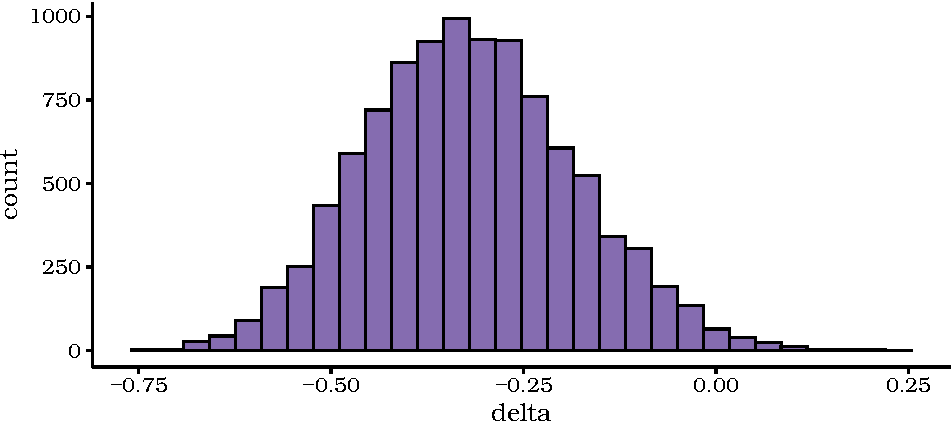
\includegraphics{manuscript_files/figure-latex/mon-1} 

}

\caption{Histogram displaying posterior of delta from Monte Carlo integration}\label{fig:mon}
\end{figure}

\hypertarget{markov-chains}{%
\section{Markov chains}\label{markov-chains}}

A Markov chain is a stochastic model expressing a sequence of possible states in which the probability of each state, \(X_{i}\), depends only on the value attained in the previous state, \(X_{i-1}\), for all \(i \geq 0\).
A Markov chain has several properties which are essential for its application in Bayesian statistics.
Definition \ref{def:markov} formalizes the requirements for a Markov chain \citep[ \text{Sec} 23.2]{Wasserman2004}.

\begin{definition}[Markov chain]
\protect\hypertarget{def:markov}{}{\label{def:markov} \iffalse (Markov chain) \fi{} }\emph{A discrete sequence of random variables \({X_{0},X_{1},...,X_{i}}\) is a Markov chain iff it satisfies the Markov property; that is, for all \(i\) and \(x \in X\):}
\[P(X_{i}=x|X_{0},...X_{i-1})=P(X_{i}=x|X_{i-1})\]
\end{definition}

A Markov chain is often represented as a directed, weighted graph where possible states are represented as vertices, and edges represent possible transitions between states. The edge weights are the conditional probabilities of the next state of the chain being the one corresponding to the edge target vertex, given that the correct state is the one corresponding to the edge source vertex.
These probabilities are also known as transition probabilities.
Markov chains also feature a probability distribution on the states at each step.
The distribution on these states changes as the number of steps increases as some states become more or less likely to occur.
After sufficiently many steps, the probability of being in any given state converges to the \emph{stationary distribution}, where it remains thereafter.
While not all Markov chains feature a stationary distribution, they are guaranteed to exist assuming the chain has certain properties, such as being \emph{ergodic}.
See Wasserman, 2004, Sec 23.2 for more details regarding convergence.

\hypertarget{metropolis-hastings-mcmc}{%
\section{Metropolis-Hastings MCMC}\label{metropolis-hastings-mcmc}}

\emph{Metropolis-Hastings MCMC} is a standard algorithm for sampling from the posterior distribution to perform a Bayesian update.
While it is not always the fastest approach in practice and requires manual tuning to work effectively, Metropolis-Hastings provides a foundation for more complex algorithms such as \emph{Hamiltonian Monte Carlo} \citep{Brooks2011} with \emph{No-U-Turn sampling} \citep{Homan2014}.
To reiterate, the purpose of sampling in Bayesian inference is to draw from the posterior density to estimate \(P(\theta|data)\) for parameters \(\theta\).
The Bayesian posterior \(P(\theta|data)\), for the purposes of MCMC, is also referred to as the \emph{target distribution}.
The basic idea of Metropolis-Hastings, to return to the previously mentioned example of approximating \(I=\int h(x)f(x)dx\), is to construct a Markov chain \(X_0,...,\) with a stationary distribution of \(f\).
Assuming the sequence has sufficiently many observations, the law of large numbers applies and the following convergence holds.
\[\frac{1}{N}\sum_{i=0}^{N}h(X_{i})\xrightarrow{P} E(h(X))=I\]
The Metropolis-Hastings algorithm provides a method for sampling from the stationary distribution of a Markov chain designed in such a way that this distribution approximates the posterior distribution.
Initially, the probability of realizing a state as part of the sampled sequence is skewed, but importantly, over time the sequence will converge to the stationary distribution, i.e., to the posterior.
Critically, the law of large numbers guarantees that with sufficiently many iterations of Metropolis-Hastings, the generated sequence of states will converge on this stationary distribution.
Essentially, given some sequence of states \(X_{0},X_{1},...,X_{i}\) from a Markov-Chain, where \(X_{0}\) is chosen arbitrarily, an iteration of Metropolis-Hastings produces the next state to include in the sequence.
As presented formally in Definition \ref{def:methas}, this is achieved by generating a \emph{proposal} for \(X_{i+1}\) from the \emph{proposal distribution} \(q(y|X_{i})\) and then accepting the proposal with some probability dependent on the relative, target probabilities of the current state \(X_{i}\) and the proposal \citep[ \text{Sec} 24.4]{Wasserman2004}.
\begin{definition}[Metropolis-Hastings MCMC]
\protect\hypertarget{def:methas}{}{\label{def:methas} \iffalse (Metropolis-Hastings MCMC) \fi{} }\emph{\(X_{i+1}\) is generated given \(X_{0},X_{1},...,X_{i}\) in the following manner:}

\begin{enumerate}
  \item Sample a proposal $Y$ from the proposal distribution $q(y|X_{i}) \textrm{ .}$
  \item Evaluate the acceptance probability $$ r(x,y)=min \{\frac{f(y)}{f(x)} \frac{q(x|y)}{q(y|x)} ,1 \} \textrm{ .}$$
  \item Compute the next state $X_{i+1}$, where $$X_{i+1}=\begin{cases}Y & \textrm{with probability }r \\ X_{i} & \textrm{with probability }1-r \end{cases} \textrm{ .}$$
\end{enumerate}
\end{definition}

While Metropolis-Hastings may seem appealing because it is both memoryless and able to approximate very complex distributions, its downfall lies in the manual tuning of the \emph{step size} parameter necessary to achieve convergence of the stationary distribution to the target distribution in a reasonable number of iterations.
Recall that Metropolis-Hastings generates proposals by sampling from some distribution.
In the special case of \emph{random walk Metropolis-Hastings}, this is a normal distribution centered about \(X_{i}\).
Here, the standard deviation of the normal distribution, also known as the \emph{step size}, dictates the relative distance in the sample space between \(X_{i}\) and the generated proposal.
If the step size is too low, the algorithm will make very small steps and may miss key features of the target distribution, causing the stationary distribution to require a much larger number of iterations to converge on the target distribution.
On the other hand, if the step size is too large, proposals will be overwhelmingly generated from the low-probability tail regions of the distribution, again resulting in a lack of convergence and poorly representative samples from the stationary distribution.
While some methods have been proposed for automatically tuning the step size parameter \citep{Graves2011}, iterating on complex, Bayesian models to tune a parameter is not particularly efficient nor computationally feasible in many cases.
For this reason, other approximation algorithms are used in practical implementations of Bayesian inference.
One such algorithm, \emph{Hamiltonian Monte Carlo} (HMC), relies on theoretical physics to compute a latent momentum variable that is applied to a hamiltonian, effectively simulating a ball rolling around the multi-dimensional sample space \citep{Brooks2011}.
Despite the increased computational cost, this method is appealing because of its ability to generate proposals from distant regions of the stationary distribution with high acceptance probabilities.
This means that in practice, the HMC algorithm's sequence converges to the stationary distribution with far fewer iterations than traditional Metropolis-Hastings implementations.
Though HMC still requires the user to specify a step size as well as a number of steps to move the hamiltonian before considering a proposal, in practice it is much more efficient and requires fewer iterations on a model.
Additionally, a proposed extension to HMC called the \emph{No-U-Turn Sampler} (NUTS) automatically determines the number of steps and was empirically demonstrated to perform at least equally as well as standard HMC \citep{Homan2014}.
The efficient algorithms briefly covered in this chapter underpin modern applications for Bayesian inference including Stan, which are discussed in the following chapter.

\hypertarget{bayesian-inference-with-stan}{%
\chapter{Bayesian inference with Stan}\label{bayesian-inference-with-stan}}

Created at Columbia University by Bob Carpenter and Andrew Gelman, Stan is a domain-specific programming language that provides tools for specifying, executing, and evaluating statistical models.
Currently comprised of more than 45 core developers from a wide array of educational institutions, private entities, and research organizations, over the past nine years the Stan project has grown to become one of the leading options for performing Bayesian inference computationally \citep{Stan2021}.
Among the many capabilities of the Stan language, is the ability to define priors, specify dependencies between variables, and impose known limits on parameters.
After all model components have been specified, a Stan model compiles first to C++ and then to binary, which can then be executed to produce an estimation of the posterior densities of all parameters, including intermediate ones, obtained through sampling, with accompanying metadata for evaluating the sampling process.

\hypertarget{the-stan-program}{%
\section{The Stan Program}\label{the-stan-program}}

While Stan is not strictly a tool for Bayesian statistical methods, it is most often used for its efficient MCMC sampler for Bayesian inference.
In essence, Stan has a sampler that takes a model and creates a separate program that explores the sample space to learn the parameters of interest in the modeling task using what is essentially the previously mentioned NUTS HMC sampling algorithm to generate draws from the posterior distribution.
As it is written in C++ and thus produces binary code, a Stan program can take advantage of the full capabilities of the machine on which it is executed.
Theoretically, Stan allows computer scientists and statisticians to construct, evaluate, and iterate on extremely complex, hierarchical models in one consolidated environment.

A typical Stan program is comprised of several, optional \emph{program blocks}, which provide a general organizational structure to a Stan program and generally allow for the declaration of variables and accompanying statements about those variables.
Block types include functions, data, transformed data, parameters, transformed parameters, model, and generated quantities.
Each of these block types serves a different purpose in a general modeling schema; however, no block is required for the Stan compiler to execute, and an empty string is considered a valid Stan program (though it may not yield a very useful model).
After the program samples the user-specified number of iterations and completes execution, a fit object and accompanying summary statistics are produced, which allow for performing post hoc evaluation such as trace and pairs plots.

\begin{example}
\protect\hypertarget{exm:stan}{}{\label{exm:stan} }Bob, a marine biologist at Florida Fish and Wildlife, studies shifting patterns in encounters between humans and large marine wildlife.
After seeing a local news headline about a recent string of shark attacks in his town, Bob became interested in trying to determine if the rate of shark attacks from year to year in Florida is changing. To do this, Bob decides to use Bayesian inference to compute a \emph{Poisson regression} for a dataset of shark attack counts each year in Florida \citep{Collier2018}. Bayesian Poisson regression models are useful for learning parameters that take the form of a count per unit of time or space. Specifically, in a Poisson regression scenario, the data \(X_0,...,X_n\) are Poisson(\(\lambda\)), and the prior distribution (the conjugate prior of the Poisson) is a gamma distribution with shape \(\alpha\) and rate \(\beta\) parameters \citep{Hitchcock2014}. The dataset includes 54 points presented below as columns, each with 4 attributes---year, population, attacks, and fatalities---depicted as rows \citep{Simonoff2003}.
\end{example}

\begin{Shaded}
\begin{Highlighting}[]
\FunctionTok{glimpse}\NormalTok{(sharks, }\AttributeTok{width=}\DecValTok{79}\NormalTok{)}
\end{Highlighting}
\end{Shaded}

\begin{verbatim}
Rows: 54
Columns: 4
$ year       <int> 1946, 1947, 1948, 1949, 1950, 1951, 1952, 1953, 1954, 1...
$ population <int> 2473000, 2539000, 2578000, 2668000, 2771305, 2980000, 3...
$ attacks    <int> 0, 1, 0, 0, 1, 0, 3, 1, 0, 0, 1, 5, 2, 4, 2, 4, 2, 3, 7...
$ fatalities <int> 0, 1, 0, 0, 0, 0, 1, 0, 0, 0, 0, 0, 0, 1, 0, 1, 0, 0, 0...
\end{verbatim}

Bob writes the model in Stan with three blocks---data, parameters, and model.

\begin{verbatim}
data {
    int<lower=0> N;              # Number of observations in dataset
    int<lower=0> attacks[N];     # An array of attack counts
    real         year[N];        # A corresponding array of years
    int<lower=0> population[N];  # Array of population for each year
}
parameters {
    real alpha;                  # Shape parameter
    real beta;                   # Rate parameter
}                  
model {
    beta ~ normal(0.015, 0.015); # Placing a normal prior on beta
    for (n in 1:N) # Every count modeled by a log-link with a linear combination
        attacks[n] ~ poisson_log(log(population[n]) + alpha + beta * year[n]);
}
\end{verbatim}

Here, the data block is used to specify the type and quantity of data to be processed by the model.
While \(N\) could be replaced with an actual integer, keeping fields of this type allows for models to be more flexible and require fewer changes.
Additionally, the parameters block is used to declare the model's parameters, which correspond directly to the variables Stan will sample at run time \citep[ \text{Sec} 8.1]{StanManual2016}.
Finally, the model parameters block is used to define the model, which includes the specification of any custom priors and the overall model formulae.
In this case, Bob put a \(normal(0.015,0.015)\) prior on beta to include into the model his domain-specific assumption that shark attacks are occurring at increasing rates each year---specifically, that this rate is increasing at about 1.5\% each year.
After specifying the model, Bob uses the Stan compiler to compile his code and then executes it to sample his model, in this case the stan function from the rstan interface is used to combine these two steps.

\begin{Shaded}
\begin{Highlighting}[]
\NormalTok{sharks\_data }\OtherTok{=} \FunctionTok{list}\NormalTok{(}
    \StringTok{\textquotesingle{}N\textquotesingle{}} \OtherTok{=} \FunctionTok{length}\NormalTok{(sharks}\SpecialCharTok{$}\NormalTok{population),}
    \StringTok{\textquotesingle{}population\textquotesingle{}}\OtherTok{=}\NormalTok{ sharks}\SpecialCharTok{$}\NormalTok{population,}
    \StringTok{\textquotesingle{}year\textquotesingle{}}\OtherTok{=}\NormalTok{ sharks}\SpecialCharTok{$}\NormalTok{year,}
    \StringTok{\textquotesingle{}attacks\textquotesingle{}} \OtherTok{=}\NormalTok{ sharks}\SpecialCharTok{$}\NormalTok{attacks}
\NormalTok{)}
\NormalTok{shark\_fit }\OtherTok{=}\NormalTok{ rstan}\SpecialCharTok{::}\FunctionTok{stan}\NormalTok{(}\AttributeTok{model\_code =}\NormalTok{ sharks\_stancode,}
                 \AttributeTok{cores=}\DecValTok{4}\NormalTok{, }\AttributeTok{data=}\NormalTok{sharks\_data, }
                 \AttributeTok{chains=}\DecValTok{4}\NormalTok{, }\AttributeTok{iter=}\DecValTok{2000}\NormalTok{)}
\end{Highlighting}
\end{Shaded}

After his model has finished sampling, Bob first takes a look at the summary statistics.

\begin{Shaded}
\begin{Highlighting}[]
\FunctionTok{print}\NormalTok{(}\FunctionTok{summary}\NormalTok{(shark\_fit, }\AttributeTok{pars=}\FunctionTok{c}\NormalTok{(}\StringTok{\textquotesingle{}alpha\textquotesingle{}}\NormalTok{, }\StringTok{\textquotesingle{}beta\textquotesingle{}}\NormalTok{))}\SpecialCharTok{$}\NormalTok{summary, }\AttributeTok{digits=}\DecValTok{2}\NormalTok{)}
\end{Highlighting}
\end{Shaded}

\begin{verbatim}
        mean se_mean     sd    2.5%     25%    50%     75%   97.5% n_eff Rhat
alpha -73.54 0.35745 8.2343 -91.320 -78.804 -73.17 -67.829 -58.864   531    1
beta    0.03 0.00018 0.0041   0.023   0.027   0.03   0.033   0.039   531    1
\end{verbatim}

Bob notes that beta, the rate parameter he is interested in understanding, seems to be increasing by about 3\% each year, although the 97.5\% confidence interval of \textasciitilde4\% causes Bob to wonder how certain he should be in his conclusion about beta. To get a better understanding of the relative frequencies of different samples of the model's parameter values, Bob plots the sample values for each iteration on a histogram, as presented in Figure \ref{fig:hist}.

\begin{figure}

{\centering 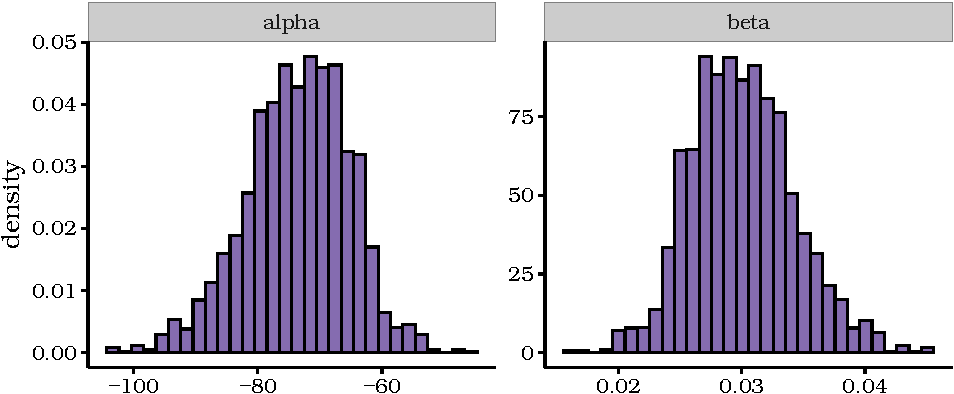
\includegraphics{manuscript_files/figure-latex/hist-1} 

}

\caption{Histograms displaying frequencies of varying sampled values for parameters alpha and beta}\label{fig:hist}
\end{figure}

The final analysis step for Bob's Bayesian model is ensuring the chains mixed properly, which Bob determines qualitatively using a trace plot as shown in Figure \ref{fig:trace}.

\begin{figure}

{\centering 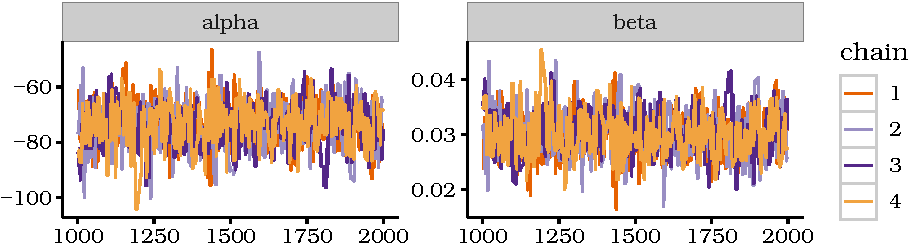
\includegraphics{manuscript_files/figure-latex/trace-1} 

}

\caption{Each chain represents a sequence of states sampled from the posterior for parameters alpha and beta. Four chains were sampled for this model, and this trace plot is a qualitative method for determining if the sample space for each parameter was sufficiently explored. Here, the sampled value of each parameter (y-axis) is plotted for every iteration (x-axis) Stan evaluated. In this case, Bob specified 2000 total iterations and 1000 burn in iterations, so the first 1000 samples were discarded and not included in the posterior or the trace.}\label{fig:trace}
\end{figure}

As it is clear the chains mixed well---each chain overlaps substantially and frequently with the other chains---Bob is now relatively confident in the results his model is producing. While he does trust the samples evaluated by his model and his analysis of Figure \ref{fig:hist}---that the rate of shark attacks is indeed increasing in Florida by some amount---the general lack of concentrated density in both histograms leads Bob to determine that he should collect more data and continue sampling his fit in an attempt to gain a better understanding of precisely how much shark attacks are increasing each year.
Stan, and more generally Bayesian inference, is a good option for a task like this because Bob can simply collect more data and continue training this model with his new data, without the need to start the fitting process over again.

\hypertarget{why-stan}{%
\section{Why Stan?}\label{why-stan}}

According to Andrew Gelman, a well-known Bayesian statistician at Columbia University, and associates, the motivation behind developing STAN was to address several shortcomings in other technologies for performing Bayesian inference, which made these alternatives impractical for learning large, complex systems \citep{Gelman2015}.
The four main shortcomings of previous software Stan's developers aimed to address were flexibility (being able to fit any given model), ease of use/ user programming time, run time, and scalability to larger datasets and more complex models \citep{Gelman2015}.
Compared to two of its most direct predecessors, Jags and Bugs, STAN is generally more flexible although notably it cannot handle discrete parameters while both Jags and Bugs can.
Stan was demonstrated to be both faster and scale better for complex models than Bugs and Jags, which the developers contribute to general efficiency in implementation, use of memory management, and most importantly the advanced MCMC algorithm STAN employs \citep{Gelman2015}.
Stan's use of HMC \citep{Brooks2011} and a slightly modified No-U-Turn sampler \citep{Homan2014}, means that it often provides large efficiency boosts compared to conventional solutions using Metropolis-Hastings or Gibbs sampling (Bugs and Jags).\\
In one example, the authors demonstrated that Stan can sample a hierarchical logistic regression model of a large dataset approximately twice as fast as Jags and produce an effective sample size of nearly four times its predecessor \citep{Gelman2015}.
While it is highly performant compared to previous options, Stan's overall performance is strongly dependent on the joint posterior of all parameters, and as we will elaborate upon in the following chapter can struggle to sample big datasets with numerous \emph{Gaussian Processes} \citep{Gelman2015}.

\hypertarget{hybrid-species-distribution-modeling-through-bayesian-inference}{%
\chapter{Hybrid species distribution modeling through Bayesian inference}\label{hybrid-species-distribution-modeling-through-bayesian-inference}}

In the field of biology and ecology, predicting the presence or absence of animal species in varying locations is a topic of much interest and critical importance for a variety of reasons.
As climate change accelerates the shifting of species' ranges \citep[\citet{Steinbauer2018}]{Parmesan2003}, understanding the dynamics of these shifts and predicting future ranges will aid researchers in understanding how best to preserve global biodiversity.
Currently, there are two main approaches for constructing \emph{species distribution models} (SDMs)---mechanistic models and correlative models \citep[\citet{Kotta2019}]{Buckley2010}.
Mechanistic models utilize explicit relationships between environmental variables and species' behaviors/ tolerances as a means for estimating species prevalence in different locations \citep[\citet{Kotta2019}]{Buckley2010}.
Correlative models, on the other hand, draw estimations by relating species' occurrences to environmental conditions in a particular area at the same time \citep[\citet{Kotta2019}]{Buckley2010}.
In their review, \citet{Buckley2010} compared predictions from several correlative and mechanistic models of the current and future distributions of two species---\emph{Atalopedes campestris}, a skipper butterfly, and \emph{Sceloporus undulatus}, a fence lizard.
Both model types performed similarly in predicting current distributions in previously unobserved locations, though the mechanistic models generally forecasted a larger future range shift in response to climate change.
While many researchers believe that correlative models have much potential for forecasting species distributions, it is becoming increasingly clear that a somewhat mechanistic approach is necessary for understanding the limits and intricacies of these ranges \citep{Kearney2006}.
As a result, a variety of hybrid modeling schemas have been proposed for incorporating domain-specific knowledge about the degree of species' tolerances to different environmental variables into the mechanistic modeling schema \citep[\citet{Kearney2006}]{Buckley2010}.

Recently, novel methods for building hybrid SDMs using Bayesian inference with \emph{Gaussian Processes} (GPs) have been proposed as a means for combining \emph{a priori} biological knowledge regarding the physical tolerance limits of species to environmental conditions with distributional data aimed at elucidating the natural variability in niche-specific environmental conditions \citep{Kotta2019}.
As previously mentioned, Bayesian inference allows for incorporating prior knowledge into the learning schema in an intuitive manner using informative priors.
Furthermore, placing priors on Gaussian processes takes advantage of the underlying flexibility of GPs, a distribution of all possible functions over a sample space with arbitrarily many dimensions.

\hypertarget{experimental-design}{%
\section{Experimental design}\label{experimental-design}}

The authors used two species native to the Baltic Sea region in a case study evaluating the efficacy of Bayesian inference as a tool for distribution modeling---\emph{Fucus vesiculosus}, a microalgae, and \emph{Idotea balthica}, a herbivore.
The authors performed this learning task in MATLAB using the GPStuff package \citep{Vanhatalo2015}, which was developed by one of the authors, Jarno Vanhatalo.
We attempted to replicate the authors' findings using the Stan programming language for two main reasons---to validate their findings and to evaluate the feasibility of constructing a complex, hierarchical model, which makes heavy use of GPs, in Stan.
The authors modeled the occurrence of each species with three separate methodologies, which were subsequently compared in both interpolation and extrapolation scenarios for accuracy.
First, the occurrence (\emph{biomass}) of each species was modeled using experimental data collected in a laboratory experiment wherein \emph{F. vesiculosus} and \emph{I. balthica} were reared in varying environmental conditions, and their survival/biomass was recorded for later use.
Additionally, the biomass of each species was modeled using distributional data combined from several sources sampled from June to August from 2005 to 2015.
Altogether, the distributional dataset features Biomass records from quantitative samples collected using a sieve from 6407 stations around the Baltic Sea.
The corresponding data for environmental variables (temperature and salinity) was sourced from the Swedish Meteorological and Hydrological Institute (SMHI) using the echam5/RCAO model and covers the entirety of the Baltic Sea at a grid resolution of 2 NM \citep{Meier2012}.
Geospatial data (depth) was ascertained from the Baltic Sea Bathymetry Database \citep{Bath2021}.
Finally, a combined model was constructed to model both experimental and distributional data together.
In each case, a \emph{hurdle model} was used to cover both presence/absence and biomass observations.
A hurdle model is a class of models where the probability of a random variable \(Y\) attaining 0 is modeled separately from the probability of attaining a non-zero value \citep[ \text{Sec } 5.6]{StanManual2016}.
All data used in our replication of \citet{Kotta2019} was ascertained directly from Jonne Kotta and Jarno Vanhatalo and can be made available upon request.

\hypertarget{implementation-with-stan}{%
\section{Implementation with Stan}\label{implementation-with-stan}}

Though we were able to sample several models with varying levels of complexity using Stan, post-sampling analysis of all resulting models revealed each to be faulty.
Here, we introduce one of the three modeling tasks \citet{Kotta2019} conducted and our implementation in BRMs, an R-based Stan interface \citep{Burkner2017}.
In our case study, the biomass of \emph{F. vesiculosus} was modeled for distribution data using environmental and geospatial covariates with a hurdle model in a hierarchical schema---the model was written in multiple levels which combine to form the complete model.
The data used in this modeling task has the following form:

\begin{verbatim}
Rows: 6,407
Columns: 6
$ Depth                 <dbl> 0.2, 1.0, 3.1, 5.0, 8.0, 2.0, 5.0, 5.0, 1.3,...
$ Salinity_current      <dbl> 7.372433, 7.371860, 7.370509, 7.370041, 7.36...
$ Temperature_current   <dbl> 15.29270, 15.21756, 15.17266, 15.13744, 15.1...
$ Fucus_vesiculosus_bio <dbl> 760.75, 26.21, 0.00, 0.00, 0.00, 11.49, 0.00...
$ POINT_X               <dbl> -113627.93, -113451.65, -113221.18, -113087....
$ POINT_Y               <dbl> 6190269, 6190859, 6190732, 6190645, 6190494,...
\end{verbatim}

Given the data, the hurdle model for \emph{F. vesiculosus} was formulated as
\[P(y_i|\pi_i,\mu_i,\tau_i^2)= \begin{cases}(1-\pi_i) & \textrm{if }y_i=0\\\ \pi_i \times N(y_i|\mu_i,\tau_i^2) & \textrm{if }y_i \in R\end{cases}\textrm{ .}\]
In this formulation, \(y_i\) is the biomass of \emph{F. vesiculosus} for any given observation i, \(\pi_i\) is the probability of occurrence of \emph{F. vesiculosus}, and \(\mu_i\) and \(\tau_i\) are the mean and variance of the Gaussian probability density function respectively.
A \emph{half Student-t} prior with 0 mean and scale 1 was put on the variance parameter, \(\tau_i\).
Both \(\pi_i\) and \(\mu_i\) were modeled using additive models.
\(\pi_i\) was represented with a logit link function---logarithm of the odds ratio of occurrence probability---as follows.
\[logit^{-1}(\pi_i)=log( \frac{\pi_i}{1-\pi_i})=\alpha+f_{ST}(x_{S,i},x_{T,i})+f_D(x_{D,i})+ \phi(s_i)\]
Finally, \(\mu_i\), the mean of the Gaussian PDF (biomass model), was represented similarly.
\[\mu_i= \alpha+f_{ST}(x_{S,i},x_{T,i})+f_D(x_{D,i})+ \phi(s_i)\]
In both cases, \(f_{ST}\) is the GP response function along temperature and salinity, and \(f_{D}\) is the GP response function along depth.
GP priors were put on \(f_{ST}\) and \(f_{D}\) with 0 mean and Gaussian covariance functions.
Additionally, \(\alpha\) is the intercept, which has \(N(0,10)\) prior, and \(\phi\) is the spatial random effect---a spatial GP with 0 mean and exponential covariance.

To formulate the model in Stan, a custom family was needed for the hurdle model.
This family was implemented in BRMs using the \texttt{custom\_family} function as reproduced here.

\begin{Shaded}
\begin{Highlighting}[]
\NormalTok{hurdle\_normal }\OtherTok{\textless{}{-}}\NormalTok{ brms}\SpecialCharTok{::}\FunctionTok{custom\_family}\NormalTok{(}
  \AttributeTok{name =} \StringTok{"hurdle\_normal"}\NormalTok{, }
  \AttributeTok{dpars =} \FunctionTok{c}\NormalTok{(}\StringTok{"mu"}\NormalTok{, }\StringTok{"hsigma"}\NormalTok{, }\StringTok{"hlogitpi"}\NormalTok{),}
  \AttributeTok{links =} \FunctionTok{c}\NormalTok{(}\StringTok{"log"}\NormalTok{, }\StringTok{"log"}\NormalTok{, }\StringTok{"identity"}\NormalTok{), }
  \AttributeTok{lb =} \FunctionTok{c}\NormalTok{(}\ConstantTok{NA}\NormalTok{, }\DecValTok{0}\NormalTok{, }\ConstantTok{NA}\NormalTok{),}
  \AttributeTok{ub =} \FunctionTok{c}\NormalTok{(}\ConstantTok{NA}\NormalTok{, }\ConstantTok{NA}\NormalTok{, }\ConstantTok{NA}\NormalTok{),}
  \AttributeTok{type =} \StringTok{"real"}\NormalTok{)}
\NormalTok{stan\_funs }\OtherTok{\textless{}{-}} \StringTok{"real hurdle\_normal\_lpdf(}
\StringTok{                real y, real mu, real hsigma, real hlogitpi) \{ }
\StringTok{    real hpi = inv\_logit(hlogitpi);}
\StringTok{    if (y == 0) \{}
\StringTok{      return bernoulli\_lpmf(0 | hpi); }
\StringTok{    \} else \{ }
\StringTok{      return bernoulli\_lpmf(1 | hpi) +  }
\StringTok{        normal\_lpdf(y | mu, hsigma);\}\}"}
\NormalTok{stanvars }\OtherTok{\textless{}{-}} \FunctionTok{stanvar}\NormalTok{(}\AttributeTok{scode =}\NormalTok{ stan\_funs, }\AttributeTok{block =} \StringTok{"functions"}\NormalTok{)}
\end{Highlighting}
\end{Shaded}

After specifying the custom \texttt{hurdle\_normal} family, the model formula was provided to Stan in the following manner.

\begin{Shaded}
\begin{Highlighting}[]
\NormalTok{formulae }\OtherTok{\textless{}{-}} 
  \FunctionTok{bf}\NormalTok{(Fucus\_vesiculosus\_bio }\SpecialCharTok{\textasciitilde{}} \FunctionTok{gp}\NormalTok{(Temperature\_current, Salinity\_current) }\SpecialCharTok{+} 
    \FunctionTok{gp}\NormalTok{(Depth) }\SpecialCharTok{+} \FunctionTok{gp}\NormalTok{(POINT\_X, POINT\_Y, }\AttributeTok{gr =} \ConstantTok{TRUE}\NormalTok{)) }\SpecialCharTok{+}
  \FunctionTok{bf}\NormalTok{(hlogitpi }\SpecialCharTok{\textasciitilde{}} \FunctionTok{gp}\NormalTok{(Temperature\_current, Salinity\_current) }\SpecialCharTok{+} \FunctionTok{gp}\NormalTok{(Depth) }\SpecialCharTok{+} 
    \FunctionTok{gp}\NormalTok{(POINT\_X, POINT\_Y, }\AttributeTok{gr =} \ConstantTok{TRUE}\NormalTok{)) }\SpecialCharTok{+}
\NormalTok{  hurdle\_normal}
\end{Highlighting}
\end{Shaded}

The \texttt{gp} function is used to specify a Gaussian process term, which gets evaluated with the rest of the model at runtime.
Similarly, the \texttt{bf} function is used to set up a model formula for input into the model through the brms interface.
Finally, the \texttt{hurdle\_normal} reference is used to specify that the custom \texttt{hurdle\_normal} family should be used in this model.
Next, the priors for each parameter were specified.
Priors mentioned thus far were taken directly from \citet{Kotta2019}.
The remaining priors were either inferred from the authors' code (available upon request), or they were set to the default prior for a given parameter type.

\begin{Shaded}
\begin{Highlighting}[]
\NormalTok{priors }\OtherTok{\textless{}{-}} \FunctionTok{c}\NormalTok{(}
  \FunctionTok{prior}\NormalTok{(}\FunctionTok{student\_t}\NormalTok{(}\DecValTok{4}\NormalTok{, }\DecValTok{0}\NormalTok{, }\DecValTok{10}\NormalTok{), }\AttributeTok{class =} \StringTok{"hsigma"}\NormalTok{),}
  \FunctionTok{prior}\NormalTok{(}\FunctionTok{normal}\NormalTok{(}\DecValTok{0}\NormalTok{, }\DecValTok{10}\NormalTok{), }\AttributeTok{class=}\StringTok{"Intercept"}\NormalTok{),}
  \FunctionTok{prior}\NormalTok{(}\FunctionTok{student\_t}\NormalTok{(}\DecValTok{4}\NormalTok{, }\DecValTok{0}\NormalTok{, }\DecValTok{1}\NormalTok{), }\AttributeTok{class=}\StringTok{"sdgp"}\NormalTok{, }
        \AttributeTok{coef=}\StringTok{"gpTemperature\_currentSalinity\_current"}\NormalTok{),}
  \FunctionTok{prior}\NormalTok{(}\FunctionTok{lognormal}\NormalTok{(}\DecValTok{2}\NormalTok{, }\FloatTok{0.2}\NormalTok{), }\AttributeTok{class=}\StringTok{"lscale"}\NormalTok{, }
        \AttributeTok{coef=}\StringTok{"gpTemperature\_currentSalinity\_current"}\NormalTok{), }
  \CommentTok{\# above values inferred from distributionData\_fucus\_v302.m:233{-}239}
  \FunctionTok{prior}\NormalTok{(}\FunctionTok{student\_t}\NormalTok{(}\DecValTok{4}\NormalTok{, }\DecValTok{0}\NormalTok{, }\DecValTok{1}\NormalTok{), }\AttributeTok{class=}\StringTok{"sdgp"}\NormalTok{, }\AttributeTok{coef=}\StringTok{"gpDepth"}\NormalTok{),}
  \FunctionTok{prior}\NormalTok{(}\FunctionTok{normal}\NormalTok{(}\DecValTok{5}\NormalTok{,}\DecValTok{1}\NormalTok{), }\AttributeTok{class=}\StringTok{"lscale"}\NormalTok{, }\AttributeTok{coef=}\StringTok{"gpDepth"}\NormalTok{),}
  \FunctionTok{prior}\NormalTok{(}\FunctionTok{student\_t}\NormalTok{(}\DecValTok{4}\NormalTok{,}\DecValTok{0}\NormalTok{,}\DecValTok{1}\NormalTok{), }\AttributeTok{class=}\StringTok{"sdgp"}\NormalTok{, }\AttributeTok{coef=}\StringTok{"gpPOINT\_XPOINT\_Y"}\NormalTok{),}
  \FunctionTok{prior}\NormalTok{(}\FunctionTok{normal}\NormalTok{(}\DecValTok{0}\NormalTok{, }\DecValTok{10}\NormalTok{), }\AttributeTok{class =} \StringTok{"Intercept"}\NormalTok{, }\AttributeTok{dpar=}\StringTok{"hlogitpi"}\NormalTok{),}
  \FunctionTok{prior}\NormalTok{(}\FunctionTok{student\_t}\NormalTok{(}\DecValTok{4}\NormalTok{, }\DecValTok{0}\NormalTok{, }\DecValTok{1}\NormalTok{), }\AttributeTok{class=}\StringTok{"sdgp"}\NormalTok{, }
        \AttributeTok{coef=}\StringTok{"gpTemperature\_currentSalinity\_current"}\NormalTok{, }\AttributeTok{dpar=}\StringTok{"hlogitpi"}\NormalTok{),}
  \FunctionTok{prior}\NormalTok{(}\FunctionTok{lognormal}\NormalTok{(}\DecValTok{2}\NormalTok{, }\FloatTok{0.2}\NormalTok{), }\AttributeTok{class=}\StringTok{"lscale"}\NormalTok{, }
        \AttributeTok{coef=}\StringTok{"gpTemperature\_currentSalinity\_current"}\NormalTok{, }\AttributeTok{dpar=}\StringTok{"hlogitpi"}\NormalTok{), }
  \CommentTok{\# above values inferred from distributionData\_fucus\_v302.m:233{-}239}
  \FunctionTok{prior}\NormalTok{(}\FunctionTok{student\_t}\NormalTok{(}\DecValTok{4}\NormalTok{, }\DecValTok{0}\NormalTok{, }\DecValTok{1}\NormalTok{), }\AttributeTok{class=}\StringTok{"sdgp"}\NormalTok{, }\AttributeTok{coef=}\StringTok{"gpDepth"}\NormalTok{, }\AttributeTok{dpar=}\StringTok{"hlogitpi"}\NormalTok{),}
  \FunctionTok{prior}\NormalTok{(}\FunctionTok{normal}\NormalTok{(}\DecValTok{5}\NormalTok{,}\DecValTok{1}\NormalTok{), }\AttributeTok{class=}\StringTok{"lscale"}\NormalTok{, }\AttributeTok{coef=}\StringTok{"gpDepth"}\NormalTok{, }\AttributeTok{dpar=}\StringTok{"hlogitpi"}\NormalTok{),}
  \FunctionTok{prior}\NormalTok{(}\FunctionTok{student\_t}\NormalTok{(}\DecValTok{4}\NormalTok{,}\DecValTok{0}\NormalTok{,}\DecValTok{1}\NormalTok{), }\AttributeTok{class=}\StringTok{"sdgp"}\NormalTok{, }\AttributeTok{coef=}\StringTok{"gpPOINT\_XPOINT\_Y"}\NormalTok{, }
        \AttributeTok{dpar=}\StringTok{"hlogitpi"}\NormalTok{))}
\end{Highlighting}
\end{Shaded}

Finally, the model was compiled and sampled using the \texttt{brm} function.

\begin{Shaded}
\begin{Highlighting}[]
\NormalTok{fit }\OtherTok{\textless{}{-}}\NormalTok{ brms}\SpecialCharTok{::}\FunctionTok{brm}\NormalTok{(}\AttributeTok{formula =}\NormalTok{ formulae, }
                 \AttributeTok{data =}\NormalTok{ Final\_Distribution\_Dataset, }
                 \AttributeTok{prior =}\NormalTok{ priors,}
                 \AttributeTok{family =}\NormalTok{ hurdle\_normal, }
                 \AttributeTok{stanvars =}\NormalTok{ stanvars)}
\end{Highlighting}
\end{Shaded}

The problems we encountered while using Stan for this task were twofold---sampling for this model took on the order of 7-14 days, and post hoc model analysis either revealed a sizable quantity of divergent transitions or that the chains had not converged.
The duration of each sampling job made testing and iterating on a model design nearly impossible given the time constraints of this project.
For models with divergent transitions, the proportion of samples with divergent transitions was so large (\textasciitilde90\%) that the model was evidently not to be trusted.
As the Stan manual notes, ``The primary cause of divergent transitions in Euclidean HMC (other than bugs in the code) is highly varying posterior curvature, for which small step sizes are too inefficient in some regions and diverge in other regions'' \citep{StanManual2016}.
Though we cannot fully exclude the possibility of bugs in our model, we reviewed our code exhaustively.
Essentially, divergent transitions occur because the sampler needs to find the ideal step size where the maximum tree depth is not causing the sampler to halt before making a U-turn too often but is also not so large as to cause sizable divergences in proposals, which occurs in the case of our model.
The issue of chains properly mixing was discussed in Example \ref{exm:stan}, and an example of insufficiently mixed chains is presented in Figure \ref{fig:nomix}.

\begin{figure}

{\centering 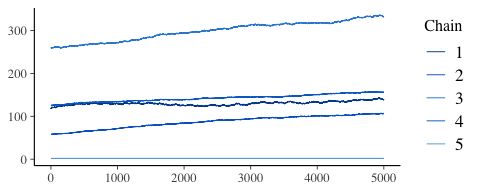
\includegraphics{manuscript_files/figure-latex/nomix-1} 

}

\caption{Each chain represents a sequence of states sampled from the posterior for the gp(Temperature, Salinity) parameter. The resultant density plot is also presented. The general lack of overlap/mixing in the chains indicates that this density plot, thus the model, should not be trusted.}\label{fig:nomix}
\end{figure}

All told, these limitations in our implementation of Kotta et al.'s (2019) model made our original goal of replicating this study in Stan a very difficult task.
Validation of our modeling setup was also made more challenging due to the homegrown nature of the code the authors provided as their implementation.
The several thousand lines of code written by the author of the GPStuff package were difficult for us to extract meaning from.
Despite these limitations, the incredibly long sampling time required to fit each model validated the underemphasized aside in \citet{Gelman2015}---Stan struggles immensely with any sort of complex GPs.
As Gelman put it, ``Gaussian processes are currently more challenging. When the number of elements of the process is large\ldots{} full Bayesian inference for Gaussian processes using Stan can become not just slow but effectively impossible''.
While Stan is currently one of the most compelling options for Bayesian inference with computing machines, the wide variation in sampling times for varying modeling schemas means it is not quite the plug-and-play solution many in the field hope it to be.

\hypertarget{conclusions-and-future-work}{%
\chapter*{Conclusions and future work}\label{conclusions-and-future-work}}
\addcontentsline{toc}{chapter}{Conclusions and future work}

Though we were largely unsuccessful in our numerous attempts to replicate and validate the seminal work presented in \citet{Kotta2019}, the aforementioned limitations suggest a closer collaboration may be needed with the original authors and perhaps a different software for implementation.
One of the most promising alternatives to Stam is Pyro, a deep universal probabilistic programming language written in Python and supported by PyTorch in the backend \citep[\citet{phan2019composable}]{bingham2018pyro}.
Pyro is currently used by many large companies including Siemens, IBM, and Uber and research groups at many universities such as Harvard, MIT, Stanford, Oxford, Cambridge, and The Broad Institute.
Given additional time and computing resources, using Pyro to implement a similar hierarchical model to the one presented in \citet{Kotta2019} would be a valuable extension to the work in this paper.
While the potential applications of Bayesian inference in varying subject fields are numerous, the sheer quantity of statistical expertise needed to design, implement, evaluate, and iterate on models of this sort makes Bayesian inference an impractical tool for many researchers at the moment.
Though domain-specific programming languages including Stan claim to lower the barrier to entry for this sort of modeling, the reality is that a sizable quantity of theoretical expertise in Bayesian statistics and practical experience with Bayesian inference is still needed to embark upon such an endeavor.
While challenging to implement without a graduate degree in statistics, Bayesian inference is an extremely promising learning methodology for problems where domain-specific knowledge can provide a partial picture of the sample space.
In the increasingly automated world we inhabit, tools such as Bayesian inference are necessary for providing learning systems with intuition that has been meticulously gathered by subject experts.

  \bibliography{references.bib,packages.bib}

\end{document}
